\documentclass[12pt]{article}
\usepackage[margin=1in]{geometry}
\usepackage[utf8]{inputenc}
\usepackage[spanish]{babel}
\usepackage{parskip}
\usepackage{setspace}
\usepackage{amsmath, amssymb}
\usepackage{graphicx}
\usepackage{hyperref} % Siempre debe ir al final.

% Opciones de Paquetes.
\decimalpoint           % {babel}
\onehalfspacing         % {setspace}
\graphicspath{{./img/}} % {graphics}: Indica ruta de donde se importan las imágenes.

% Encabezado.
\title{Clase 8. Funciones de varias variables y Derivadas parciales.}
\author{MIT 18.02: Multivariable Calculus.}
\date{}


\begin{document}

% Comandos personalizados.
%=========================================
%
%    Comandos personalizados usados en
%       los apuntes de este curso.
%
%=========================================

\newcommand{\vecmat}[1]{\mathbf{#1}}                          % Vectores o matrices en negrita en math mode.
\newcommand{\unitvec}[1]{\vecmat{\hat{#1}}}                   % Vectores unitarios.
\newcommand{\overvec}[1]{\overrightarrow{#1}}                 % Vector como segmento orientado.
\newcommand{\proy}[2]{\text{proy}_{\vecmat{#2}}{\vecmat{#1}}} % Proyección vectorial.
\newcommand{\invmat}[1]{\vecmat{#1}^{-1}}                     % Inversa de una matriz.
\newcommand{\transmat}[1]{\vecmat{#1}^{T}}                    % Transpuesta de una matriz.
\newcommand{\Adj}[0]{\text{Adj}}                              % Matriz adjunta.
\newcommand{\R}[0]{\mathbb{R}}                                % Símbolo conjunto de los números reales.
\newcommand{\N}[0]{\mathbb{N}}                                % Símbolo conjunto de los números naturales.


\maketitle

\begin{abstract}
\noindent En esta clase comenzamos a estudiar funciones multivariadas o que dependen de más de una variable. Revisamos sus características y cómo evaluar su comportamiento tanto de forma gráfica como mediante su límite. Luego nos centramos en aprender a calcular sus tasas de cambio instantáneas a partir de sus derivadas parciales.
\end{abstract}


\section{Funciones de varias variables.}

Muchos fenómenos o procesos del día a día se explican por más de un factor. Al modelarlos matemáticamente, se obtienen funciones conocidas como multivariadas o de varias variables.

Sea $D \subseteq \R^{n}$ un conjunto de $n$-tuplas\footnote{En términos generales, una tupla puede ser entendida como una lista ordenada finita de elementos (a diferencia de una sucesión, que puede ser infinita). Cuando ésta tiene $n$ elementos, se la denota como $n$-tupla.}. Una \textbf{función de varias variables} $f:D \to \R$ es una regla que asigna un único valor real a cada $n$-tupla de su dominio $D$. La imagen de cada $(x_{1}, \ \ldots, \ x_{n})$ bajo $f$ se denota como $f(x_{1}, \ \ldots, \ x_{n})$ y su rango es el conjunto $\{f(x_{1}, \ \ldots, \ x_{n}) \ | \ (x_{1}, \ \ldots, \ x_{n}) \in D\} \subseteq \R$.

En este curso nos centraremos en funciones bivariadas $z = f(x, \ y)$, pero todo lo que aprendamos es replicable a aquellas de más variables.

\subsection{Dominio de una función.}

En ocasiones, una función de varias variables puede ser representada como una ecuación. Dependiendo de su expresión, muchas veces tendremos que restringir su dominio para que cumpla con asignar a cada elemento de este conjunto un único valor de su codominio.

\ejemplo Determine el dominio de las siguientes funciones:

\begin{enumerate}
\item[(a)] $f(x, y) = x^{2} + y^{2}$
\item[(b)] $g(x, y) = x \cdot \ln(y^{2} - x)$
\item[(c)] $\displaystyle h(x, y) = \frac{\sqrt{x + y + 1}}{x - 1}$
\end{enumerate}

\solucion En (a), el dominio de $f(x, \ y)$ es el conjunto $\R^{2}$ o, en otras palabras:
\[
  \text{dom}(f) = \{(x, \ y) \in \R^{2}\}
\]
En cuanto a (b), debemos restringir el dominio de $g(x, \ y)$ para que excluya a todos los pares ordenados $(x, \ y)$ donde se cumpla la desigualdad $y^{2} - x \leq 0$, puesto que $\ln(x)$ no está definido en $\R$ para todo $x \leq 0$. Por lo tanto, solo se considerarán aquellos en los que:
\begin{align*}
y^{2} - x &> 0 \\
y^{2} &> x
\end{align*}
Así,
\[
  \text{dom}(g) = \{(x, \ y) \in \R^{2} \ | \ x < y^{2}\}
\]
Finalmente, para la función $h(x, \ y)$ en (c) debemos establecer dos restricciones para su dominio. La primera es que $x + y + 1 \geq 0$, lo que es igual a:
\[
  x + y \geq -1
\]
La segunda restricción es que $x - 1 \neq 0$. Es decir,
\[
  x \neq 1
\]
De este modo,
\[
  \text{dom}(h) = \{(x, \ y) \in \R^{2} \ | \ x + y \geq -1 \text{ y } x \neq 1\}
\]

\subsection{Combinación de funciones y funciones compuestas.}

Así como con las funciones univariadas, las multivariadas también pueden ser combinadas por medio de operaciones aritméticas, tal como se observa con $f(x, \ y)$ y $g(x, \ y)$:

\begin{itemize}
\item $(f \pm g)(x, \ y) = f(x, \ y) \pm g(x, \ y)$.
\item $(f \cdot g)(x, \ y) = f(x, \ y) \cdot g(x, \ y)$.
\item $\displaystyle \left(\frac{f}{g}\right)(x, \ y) = \frac{f(x, \ y)}{g(x, \ y)}$, para $g(x, \ y) \neq 0$.
\end{itemize}

Sin embargo, \textbf{no es posible formar funciones compuestas} entre dos de varias variables. Para ello, al menos una de ellas debe ser univariada.

Por ejemplo, sean dos funciones $f(x)$ y $g(x, \ y)$. Entonces,
\[
  (f \ o \ g)(x, \ y) = f(g(x, \ y))
\]

\subsection{Formas de visualizar una función de dos variables.}

Es habitual graficar funciones de una variable al estudiar su comportamiento con respecto a los valores de su dominio. Sin embargo, esta tarea se vuelve compleja cuando depende de más factores. A pesar de esta dificultad, en esta sección veremos dos formas de visualizar funciones bivariadas: Mediante su superficie y usando gráficos de contornos.

\subsubsection{Superficie de una función.}

Una forma de visualizar funciones de dos variables es graficando sus puntos en un espacio euclidiano de tres dimensiones, donde la figura que se obtiene usualmente es una \textbf{superficie}.

Cada coordenada de una función $z = f(x, \ y)$ graficada en un espacio euclidiano es expresada como un triple (o $3$-tupla) de la forma $(x, \ y, \ z)$ o $(x, \ y, \ f(x, \ y))$.

Cuando una de las dos variables de una función es constante, obtenemos un plano. Abajo vemos el caso de $f(x, \ y) = -y$.

\begin{figure}[hbt!]
\centering
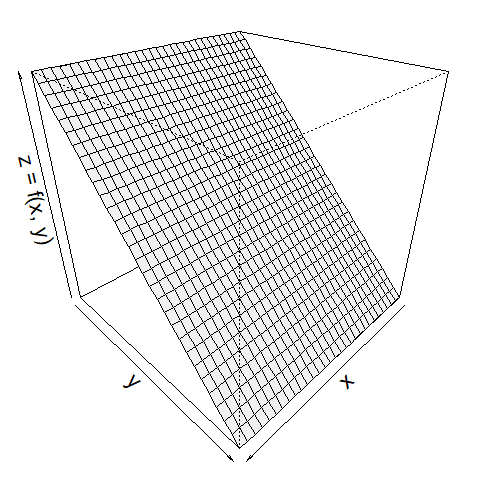
\includegraphics[scale = 0.35]{plano_var_cte.png}
\caption{Superficie de $f(x, \ y) = -y$}
\end{figure}

\newpage

La gráfica de $f(x, \ y) = -y$ es un tanto sencilla de graficar a mano, pero cuando consideramos que tanto $x$ como $y$ varían, dicho proceso se vuelve más complejo. A continuación lo vemos en $g(x, \ y) = 1 - x^{2} - y^{2}$.

\begin{figure}[hbt!]
\centering
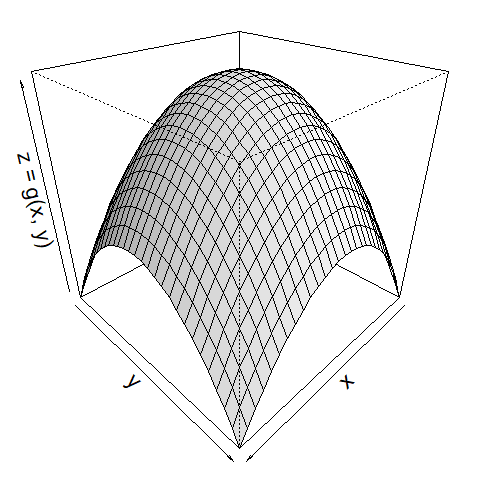
\includegraphics[scale = 0.35]{superficie.png}
\caption{Superficie de $g(x, \ y) = 1 - x^{2} - y^{2}$}
\end{figure}

Si necesitamos bosquejar a mano un gráfico como el de $g(x, \ y)$ de arriba, podemos hacerlo mediante las curvas de las ecuaciones que se obtienen de la función al definir cada variable como igual a cero. Al unir los tres planos obtenemos la figura final.

\subsubsection{Gráficos de contorno y curvas de nivel.}

Otra manera de visualizar funciones bivariadas es mediante \textbf{gráficos de contorno}, que consiste de figuras llamadas \textbf{curvas de nivel} formadas por todos los puntos $(x, \ y)$ para los cuales $f(x, \ y)$ es igual a una constante $k$. A continuación tenemos uno de $g(x, \ y) = 1 - x^{2} - y^{2}$.

\begin{figure}[hbt!]
\centering
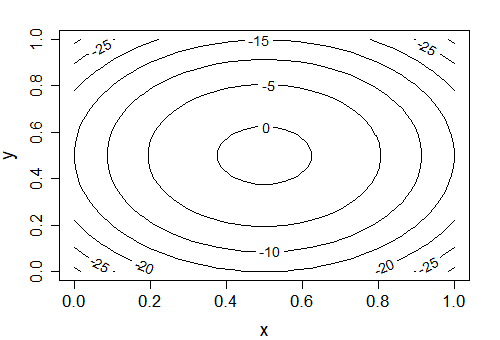
\includegraphics[scale = 0.45]{contorno-01.png}
\caption{Gráfico de contorno de $g(x, \ y) = 1 - x^{2} - y^{2}$}
\end{figure}

Como se observa en el gráfico de contorno de $g(x, \ y)$, sus curvas de nivel son círculos que se forman con ella al mantenerla fija para un valor de su rango, los que corresponden a los números que aparecen sobre estas figuras. Por ejemplo, la de $g(x, \ y) = -5$ está dada por todos los $(x, \ y)$ de su dominio donde se cumpla que $-5 = 1 - x^{2} - y^{2}$.

Las curvas de nivel pueden ser entendidas como rebanadas de la superficie de una función $f(x, \ y)$ cortadas por planos $f(x, \ y) = z$, con $z$ constante, paralelos al plano $xy$.

\begin{figure}[hbt!]
\centering
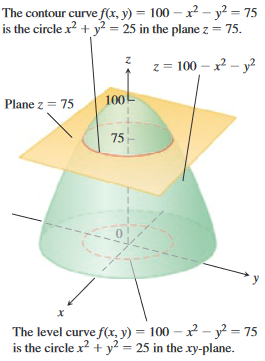
\includegraphics[scale = 0.55]{contorno-02.png}
\caption{Hass, et al (2019). \textit{Thomas Calculus. Early Transcendentals in SI Units}. Pp 774.}
\end{figure}

En ese sentido, el gráfico de contorno de $f(x, \ y)$ son todas las curvas de nivel (o rebanadas) apiladas una sobre otra.

Una ventaja de los gráficos de contorno es que facilitan el análisis de superficies generadas por funciones más complejas. Veámoslo en $h(x, \ y) = y^{2} - x^{2}$.

\begin{figure}[hbt!]
\centering
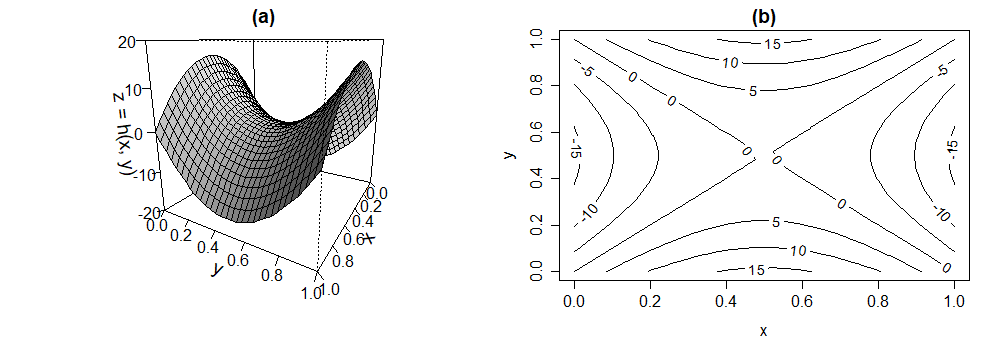
\includegraphics[scale= 0.45]{contorno-03.png}
\caption{(a) Superficie y (b) gráfico de contorno de $h(x, \ y) = y^{2} - x^{2}$}
\end{figure}

El gráfico de contorno de $h(x, \ y)$ (b) permite identificar la existencia de un aparente \textbf{punto de silla} (\textit{saddle point}) en su centro, que es un punto crítico de su función, pero no un extremo local\footnote{Más adelante los estudiaremos, pero es claro que se pueden identificar usando derivadas.}. En este caso, con respecto a $y$ es un valor mínimo, pero a lo largo de $x$ es un valor máximo. Estos no siempre son fáciles de encontrar con superficies como la de (a).

\subsection{Límite de una función de varias variables.}

También es posible estudiar el comportamiento de una función evaluando su límite. Recordemos su definición precisa o ``definición $\delta-\epsilon$'' (delta-epsilon) con funciones univariadas.

Sean $f(x)$ una función e $I$ un intervalo abierto en $x$ que contiene a $x_{0}$ con $x \neq x_{0}$. La definición $\delta - \epsilon$ señala que:
\[
  \lim_{x \to x_{0}} f(x) = L
\]
si para cada $\epsilon > 0$ existe un correspondiente $\delta > 0$ tal que:
\[
  \text{si } 0 < |x - x_{0}| < \delta, \text{ entonces } |f(x) - L| < \epsilon
\]
Es decir, el $\lim_{x \to x_{0}} f(x)$ existe si esta función está adentro del intervalo $(L - \epsilon, \ L + \epsilon)$ cuando $x \neq x_{0}$ está en $(x_{0} - \delta, \ x_{0} + \delta)$, para cualquier $\delta(\epsilon) > 0$.\footnote{Debemos escoger un $\delta$ a partir del $\epsilon$ elegido para que, efectivamente, $\lim_{x \to x_{0}} f(x) = L$.}

Para aplicar la definición $\delta-\epsilon$ del límite de una función de dos variables, antes debemos manejar los conceptos de ``punto interior'' y ``punto de frontera''.

\subsubsection{Puntos interior y de frontera.}

Sea $R \subseteq \R^{2}$ una región. El centro de un disco $(x_{0}, \ y_{0}) \in \R^{2}$ es un \textbf{punto interior} de $R$ si todos los elementos de esta figura son parte de $R$. En cambio, es un \textbf{punto de frontera} (\textit{boundary point}) si algunos de ellos (incluyendo o no a $(x_{0}, \ y_{0})$) no pertenecen a $R$.

\begin{figure}[hbt!]
\centering
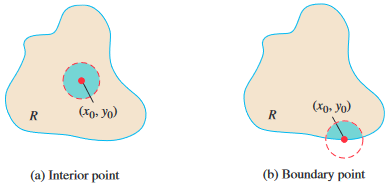
\includegraphics[scale = 0.8]{puntos-interior-frontera-01.png}
\caption{Hass, et al (2019). \textit{Thomas Calculus. Early Transcendentals in SI Units}. Pp 773.}
\end{figure}

La región $R$ se puede interpretar como el \textbf{dominio} de $f(x, \ y)$. Siguiendo la analogía de los intervalos en las funciones univariadas, $R$ es \textbf{abierto} si consiste solo de puntos interiores y es \textbf{cerrado} si se constituye solo de puntos de frontera.

A continuación vemos la región de una función bivariada que, geométricamente, corresponde a un disco unitario.

\begin{figure}[hbt!]
\centering
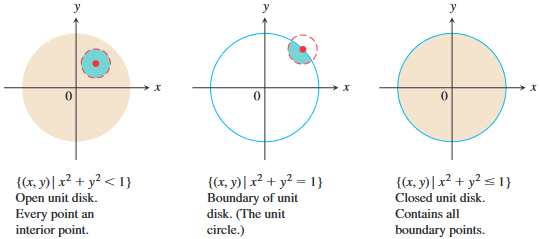
\includegraphics[scale = 0.6]{puntos-interior-frontera-02.png}
\caption{Hass, et al (2019). \textit{Thomas Calculus. Early Transcendentals in SI Units}. Pp 773.}
\end{figure}

Como se observa en el segundo disco unitario de la figura de arriba, todos los puntos de frontera de una región conforman el conjunto llamado \textbf{frontera}, mientras que el conjunto de todos los puntos interiores se conoce como \textbf{interior}.

Una región también puede abierta y cerrada a la vez si consiste tanto de puntos interiores como de fronteras. Es la misma idea de las funciones de una variable cuando su dominio está dado por un intervalo $(a, \ b]$ o $[a, \ b)$.

\subsubsection{Definición del límite de una función de dos variables.}

Sean $f(x, \ y)$ una función real, $D \subseteq \R^{2}$ su dominio (o región) y $(x_{0}, \ y_{0}), \ (x, \ y) \in D$ dos puntos, con $(x, \ y) \neq (x_{0}, \ y_{0})$. El límite de $f(x, \ y)$ mientras $(x, \ y)$ se acerca a $(x_{0}, \ y_{0})$ \textbf{existe} o, en otras palabras,
\[
  \limbiv{x_{0}, \ y_{0}} f(x, \ y) = L
\]
si para un $\epsilon > 0$ hay un correspondiente $\delta > 0$ tal que
\[
  \text{si } 0 < \sqrt{(x - x_{0})^{2} + (y - y_{0})^{2}} < \delta,
  \text{ entonces } |f(x, \ y) - L| < \epsilon
\]
Esta definición del límite de $f(x, \ y)$ indica que este valor existe si $|f(x, \ y) - L| \to 0$ cuando la distancia entre $(x, \ y)$ y $(x_{0}, \ y_{0})$ dada por la norma euclidiana $\sqrt{(x - x_{0})^{2} + (y - y_{0})^{2}} \to 0$.

Una forma de explicar esta definición $\delta-\epsilon$ del límite es que, cuando existe, podemos encontrar un disco $D_{\delta} \subseteq D$ de radio $\delta > 0$, centro $C(x_{0}, \ y_{0})$ y con $(x, \ y) \in D_{\delta}$ para cualquier intervalo pequeño $(L - \epsilon, \ L + \epsilon)$ que incluye a $L$ tal que, al aplicar a $f(x, \ y)$ sobre $D_{\delta}$, para cada punto (excluyendo posiblemente a $(x_{0}, \ y_{0})$) obtenemos un único valor en $(L - \epsilon, \ L + \epsilon)$.

\begin{figure}[hbt!]
\centering
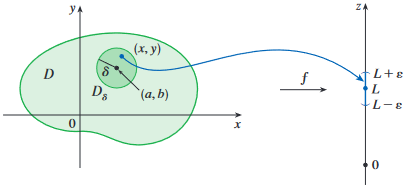
\includegraphics[scale = 0.57]{limite-funcion-bivariada.png}
\caption{Stewart, et al (2021). \textit{Calculus: Early Transcendentals}. Pp 953.}
\end{figure}

En la imagen de arriba, el punto $(x_{0}, \ y_{0}) = (a, \ b)$ es uno interior, pero también puede ser uno de frontera a pesar de que, en dicho caso, puede estar afuera de $D$. Por otra parte, siempre se debe cumplir que todos los $(x, \ y) \in D$ para que exista el $\limbiv{x_{0}, \ y_{0}} f(x, \ y)$.

\subsubsection{Cálculo y evaluación del límite de una función de dos variables.}

Mientras una función $f(x, \ y)$ no se indetermine en $(x_{0}, \ y_{0})$, podemos calcular su límite como el valor de salida en ese punto. Si es una combinación entre $g(x, \ y)$ y $h(x, \ y)$ tal que
\[
  \limbiv{x_{0}, \ y_{0}} g(x, \ y) = L
  \quad \text{y} \quad
  \limbiv{x_{0}, \ y_{0}} h(x, \ y) = M
\]
entonces se pueden utilizar las reglas (o propiedades) que se observan en la siguiente tabla:

\begin{table}[hbt!]
\centering

\renewcommand{\arraystretch}{1.5}

\begin{tabular}{c c}
\hline
\textbf{Regla} & \textbf{Fórmula} \\
\hline
Suma (y diferencia) & $\displaystyle \limbiv{x_{0}, \ y_{0}} [g(x, \ y) \pm h(x, \ y)] = L \pm M$ \\
Múltiplo constante & $\displaystyle \limbiv{x_{0}, \ y_{0}} k \cdot g(x, \ y) = k \cdot L$ \\
Producto & $\displaystyle \limbiv{x_{0}, \ y_{0}} [g(x, \ y) \cdot h(x, \ y)] = L \cdot M$ \\
Cociente & $\displaystyle \limbiv{x_{0}, \ y_{0}} \frac{g(x, \ y)}{h(x, \ y)} = \frac{L}{M} \iff M \neq 0$ \\
Potencia & $\displaystyle \limbiv{x_{0}, \ y_{0}} [g(x, \ y)]^{n} = L^{n} \iff n > 0$ \\
Raíz & $\displaystyle \limbiv{x_{0}, \ y_{0}} \sqrt[n]{g(x, \ y)} = \sqrt[n]{L} = L^{1/n} \iff n > 0$ \\
\hline
\end{tabular}

\end{table}

A las anteriores propiedades también se pueden añadir los límites especiales:
\[
  \limbiv{x_{0}, \ y_{0}} x = x_{0}; \qquad
  \limbiv{x_{0}, \ y_{0}} y = y_{0}; \qquad
  \limbiv{x_{0}, \ y_{0}} c = c
\]
Al trabajar con el límite de una función en un punto, también se puede evaluar si existe en ese lugar. Esta tarea es más compleja en aquellas que dependen de más de una variable.

Como se recordará, el límite de una función $f(x)$ en un punto existe si sus límites de la izquierda y derecha\footnote{También conocidos como límites unilaterales.} son iguales en aquel lugar. Para las multivariadas debemos hacer la misma evaluación, pero en infinitas trayectorias que pueden ser tanto lineales como curvadas\footnote{En las univariadas solo debemos evaluar dos trayectorias lineales (izquierda y derecha).}.

Por lo tanto, lo más fácil es evaluar si el límite de $f(x, \ y)$ en un punto no existe. Si hacemos lo contrario, debemos considerar la posibilidad de que para al menos una trayectoria obtengamos un valor distinto de las otras que hayamos evaluado.

Otras formas de evaluar la (no) existencia del límite de $f(x, \ y)$, es usando su definición $\delta - \epsilon$ o mediante el teorema de compresión. Todo esto lo veremos en los siguientes ejemplos.

\ejemplo Calcule el siguiente límite.
\[
  \limbiv{0, \ 1} \frac{x - xy + 3}{x^{2}y + 5xy - y^{3}}
\]
\solucion Para mayor legibilidad, establezcamos que:
\[
  h(x, \ y) = \frac{f(x, \ y)}{g(x, \ y)} = \frac{x - xy + 3}{x^{2}y + 5xy - y^{3}}
\]
Luego, calculemos los límites de $f(x, \ y)$ y $g(x, \ y)$ de manera separada.
\begin{align*}
  \limbiv{0, \ 1} f(x, \ y) &= \limbiv{0, \ 1} x - xy + 3 = 0 - (0)(1) + 3 = 3 \\ \\
  \limbiv{0, \ 1} g(x, \ y) &= \limbiv{0, \ 1} x^{2}y + 5xy - y^{3} = (0^{2})(1) + (5)(0)(1) - 1^{3} = -1
\end{align*}
De este modo, por la regla del cociente se obtiene que:
\[
  \limbiv{0, \ 1} h(x, \ y) = \limbiv{0, \ 1} \frac{x - xy + 3}{x^{2}y + 5xy - y^{3}}
                            = \frac{3}{(-1)}
                            = -3
\]

\ejemplo Calcule
\[
  \limbiv{0, \ 0} \frac{x^{2} - xy}{\sqrt{x} - \sqrt{y}}
\]
\solucion Si sustituímos directamente a $(0, \ 0)$ en la función del límite, se obtiene una forma indeterminada:
\[
  \limbiv{0, \ 0} \frac{x^{2} - xy}{\sqrt{x} - \sqrt{y}} = \frac{0^{2} - (0)(0)}{\sqrt{0} - \sqrt{0}}
                                                         = \frac{0}{0}
\]
Cuando esto ocurre, una estrategia es realizar operaciones algebraicas que no alteren a la función original. Por ejemplo, acá es posible multiplicar la función por $(\sqrt{x} - \sqrt{y})/(\sqrt{x} - \sqrt{y})$.
\[
  \frac{x^{2} - xy}{\sqrt{x} - \sqrt{y}} \cdot \left(\frac{\sqrt{x} - \sqrt{y}}{\sqrt{x} - \sqrt{y}}\right) =
    \frac{x(x - y)(\sqrt{x} - \sqrt{y})}{x - y} = x(\sqrt{x} - \sqrt{y})
\]
Así, se puede concluir que
\[
 \limbiv{0, \ 0} \frac{x^{2} - xy}{\sqrt{x} - \sqrt{y}} = \limbiv{0, \ 0} x(\sqrt{x} - \sqrt{y}) = 0
\]

\ejemplo Evalúe si existe el siguiente límite.
\[
  \limbiv{0, \ 0} \frac{3x^{2}y}{x^{2} + y^{2}}
\]
\solucion Una manera de evaluar la existencia de este límite es haciéndolo en algunas de sus trayectorias. Por ejemplo, a lo largo de $x$ o cuando $y = 0$, se obtiene que:
\[
  \frac{3x^{2}0}{x^{2} + 0^{2}} = \frac{0}{x^{2}} = 0
\]
Y a lo largo de $y$ o cuando $x = 0$:
\[
  \frac{3(0^{2})y}{0^{2} + y^{2}} = \frac{0}{y^{2}} = 0
\]
Los límites de ambas trayectorias serán iguales a $0$ mientras $(x, \ y) \to (0, \ 0)$. Esto no nos permite concluir que el límite de la función de este ejemplo existe y es igual a cero, ya que es posible que en otra obtengamos un valor distinto. Por lo tanto, tomaremos otra estrategia.

Usemos la definición $\delta - \epsilon$ para demostrar que el límite de este ejemplo existe. Sean $\epsilon > 0$ y $\delta(\epsilon) > 0$. Si:
\[
0 < \sqrt{(x - 0)^{2} + (y - 0)^{2}} = \sqrt{x^{2} + y^{2}} < \delta
\]
Y, como consecuencia,
\[
  \left|\frac{3x^{2}y}{x^{2} + y^{2}} - L\right| < \epsilon
\]
Entonces:
\[
  \limbiv{0, \ 0} \frac{3x^{2}y}{x^{2} + y^{2}} = L
\]
Debido que para las trayectorias de $x$ e $y$ vimos que el límite de esta función es igual a cero, tomemos la apuesta de que $L = 0$. Esto implica que:
\[
  \left|\frac{3x^{2}y}{x^{2} + y^{2}} - 0\right| = \left|\frac{3x^{2}y}{x^{2} + y^{2}}\right| < \epsilon
\]
El valor absoluto de esta desigualdad podemos expresarlo como:
\[
  \left|\frac{3x^{2}y}{x^{2} + y^{2}}\right| = \left(\frac{x^{2}}{x^{2} + y^{2}}\right) \cdot 3|y|
\]
La expresión $\left(\frac{x^{2}}{x^{2} + y^{2}}\right)$ es una fracción propia y en estas siempre se cumple que:
\[
  \left(\frac{x^{2}}{x^{2} + y^{2}}\right) \leq 1
\]
Por lo tanto, podemos asumir que:
\[
  \left(\frac{x^{2}}{x^{2} + y^{2}}\right) \cdot 3|y| \leq 3|y|
\]
Por otra parte $|y| = \sqrt{y^{2}}$ y $\sqrt{y^{2}} \leq \sqrt{x^{2} + y^{2}}$. Por lo tanto, podemos reescribir la desigualdad de arriba como:
\[
  \left(\frac{x^{2}}{x^{2} + y^{2}}\right) \cdot 3|y| \leq 3 \sqrt{x^{2} + y^{2}}
\]
Debido a que $\sqrt{x^{2} + y^{2}} < \delta$, podemos realizar otro reemplazo:
\[
  \left(\frac{x^{2}}{x^{2} + y^{2}}\right) \cdot 3|y| < 3 \delta
\]
Como el lado izquierdo de esta expresión es estrictamente menor a $3 \delta$, podemos asumir que:
\[
  3 \delta = \epsilon
\]
Reescribamos el lado izquierdo de la desigualdad en su forma original.
\[
  \left|\frac{3x^{2}y}{x^{2} + y^{2}} - 0\right| < 3 \delta
\]
Recordemos que el valor de $\delta$ debe estar en función de $\epsilon > 0$. Así, si escogemos un $\delta = \epsilon/3$, entonces:
\[
  \left|\frac{3x^{2}y}{x^{2} + y^{2}} - 0\right| < 3 \left(\frac{\epsilon}{3}\right) = \epsilon
\]
Esto nos permite concluir a partir de la definición $\delta - \epsilon$ que:
\[
  \limbiv{0, \ 0} \frac{3x^{2}y}{x^{2} + y^{2}} = 0
\]
Este ejemplo también se puede resolver con el \textbf{teorema de compresión} (\textit{squeeze theorem}).

Sean $I \subseteq \R$ un intervalo y $f, \ g, \ h \in \R$ funciones definidas en $I$, pero posiblemente no en $x_{0} \in I$. Para todo $(x \neq x_{0}) \in I$, el teorema de compresión señala que si:

\begin{itemize}
\item $g(x) \leq f(x) \leq h(x)$
\item $\displaystyle \lim_{x \to x_{0}} g(x) = \lim_{x \to x_{0}} h(x) = L$
\end{itemize}

entonces:
\[
  \lim_{x \to x_{0}} f(x) = L
\]
Este teorema se aplica de la misma manera en funciones de varias variables\footnote{Y también en sucesiones.}.

Anteriormente, mediante la definición $\delta-\epsilon$ del límite observamos que:
\[
  \left(\frac{x^{2}}{x^{2} + y^{2}}\right) \cdot 3|y| = \left|\frac{3x^{2}y}{x^{2} + y^{2}}\right| \leq 3|y|
\]
La desigualdad no estricta de arriba es lo mismo que:
\[
  -3|y| \leq \frac{3x^{2}y}{x^{2} + y^{2}} \leq 3|y|
\]
Los dos extremos de esta desigualdad compuesta son funciones bivariadas con $x$ constante. Al tomar sus límites mientras $(x, \ y) \to (0, \ 0)$ se obtiene:
\[
 \limbiv{0, \ 0} (-3|y|) = \limbiv{0, \ 0} 3|y| = 0
\]
De este modo, por el teorema de compresión se puede concluir que:
\[
  \limbiv{0, \ 0} \frac{3x^{2}y}{x^{2} + y^{2}} = 0
\]

\subsubsection{Continuidad de una función de varias variables.}

Al igual que en las funciones univariadas, en las de varias variables también es posible usar su límite para evaluar si es (o no) \textbf{continua} en un punto o en todo su dominio. Un caso de las primeras la vimos en el Ejemplo 2 resuelto en la sección 1.4.3.

Una función $f:D \to \R$, con $D \subseteq \R^{2}$, es \textbf{continua} en un punto $(x_{0}, \ y_{0}) \in D$ si:

\begin{enumerate}
\item $f$ está definida en $(x_{0}, \ y_{0})$.

\item $\displaystyle \limbiv{x_{0}, \ y_{0}} f(x, \ y)$ existe.

\item $\displaystyle \limbiv{x_{0}, \ y_{0}} f(x, \ y) = f(x_{0}, \ y_{0})$
\end{enumerate}

Si las condiciones de arriba se aplican a todos los $(x, \ y) \in D$, se concluye que la función $f$ es \textbf{continua en todo su dominio}.

En general, las funciones \textbf{polinómicas y racionales} siempre son \textbf{continuas en todo su dominio}. Para las primeras, dicho conjunto suele ser $\R^{n}$ y en las segundas es posible que sea uno restringido a aquellas con denominador distinto de cero.

La definición de continuidad se aplica a puntos de su dominio que son tanto interior como de frontera. La principal condición es que todos los $(x, \ y)$ cercanos a $(x_{0}, \ y_{0})$ deben ser parte de ese conjunto.


\section{Diferenciación parcial.}

Para medir cómo cambia una función multivariada en cada valor de su dominio, se calcula su derivada con respecto a una de sus variables mientras al resto de ellas se las mantiene fijas. Este proceso se conoce como \textbf{diferenciación parcial}.

\subsection{Definición del límite de las derivadas parciales de una función.}

Sea $f:D \to \R$ una función con dominio $D \subseteq \R^{2}$. Sus derivadas parciales con respecto a $x$ e $y$ en un punto $(x_{0}, \ y_{0})$ se definen como:
\begin{align*}
  (1) \ \pderivpar{x}{f(x, \ y)}{(x_{0}, \ y_{0})} &= \lim_{h \to 0} \frac{f(x_{0} + h, \ y_{0}) - f(x_{0}, \ y_{0})}{h} \\ \\
  (2) \ \pderivpar{y}{f(x, \ y)}{(x_{0}, \ y_{0})} &= \lim_{h \to 0} \frac{f(x_{0}, \ y_{0} + h) - f(x_{0}, \ y_{0})}{h}
\end{align*}
siempre que \textbf{los límites existan}, donde $h = \Delta x$ en (1), $h = \Delta y$ en (2).

Las igualdades (1) y (2) son las definiciones del límite de la derivada parcial de $f(x, \ y)$ en $(x, \ y) = (x_{0}, \ y_{0})$ con respecto a $x$ e $y$, respectivamente. Sus lados derechos calculan la tasa de cambio instantánea de esta función mientras $x \to x_{0}$ en (1) e $y \to y_{0}$ en (2).

El símbolo $\partial$ se lee como ``parcial'', mientras que los lados izquierdos de las igualdades de arriba se expresan como:
\begin{align*}
  \derivpar{x} f(x, \ y) \Longrightarrow \text{Derivada parcial de } f(x, \ y) \text{ con respecto a } x. \\ \\
  \derivpar{y} f(x, \ y) \Longrightarrow \text{Derivada parcial de } f(x, \ y) \text{ con respecto a } y.
\end{align*}
Algunas de las notaciones alternativas de la derivada parcial de una función son:
\[
% No hice otro comando similar a \pderivpar para este caso porque dudo que lo use en otras ocasión.
  f_{x}(x_{0}, \ y_{0}) = D_{x} f(x_{0}, \ y_{0}) = \left. \derivpar[f(x, \ y)]{x} \right|_{(x_{0}, \ y_{0})}
\]

\subsection{Interpretaciones de la derivada parcial.}

Al calcular la derivada parcial de $f(x, \ y)$ con respecto a $x$ en $(x_{0}, \ y_{0})$, se está manteniendo constante a $y$ en $y_{0}$. Es decir, al aplicar esta operación, se está tratando a la función bivariada como una univariada $f(x, \ y_{0})$. Por lo tanto, la tasa de cambio instantánea de la primera puede ser interpretada como la \textbf{derivada ordinaria}\footnote{Así llamaré a las derivadas de funciones univariadas para diferenciarlas de las parciales.} de la segunda en $x = x_{0}$.
\[
  \pderivpar{x}{f(x, \ y)}{(x_{0}, \ y_{0})} = \left. \deriv{x}{f(x, \ y_{0})}\right|_{x = x_{0}}
\]
Geométricamente, $f_{x}(x_{0}, \ y_{0})$ se interpreta como el valor (aproximado) de la pendiente de la recta tangente en $(x_{0}, \ y_{0}, \ f(x_{0}, \ y_{0}))$ de una curva $f(x, \ y_{0})$ ubicada en un plano $y = y_{0}$ que corta a la superficie $f(x, \ y)$ en ese punto.

\begin{figure}[hbt!]
\centering
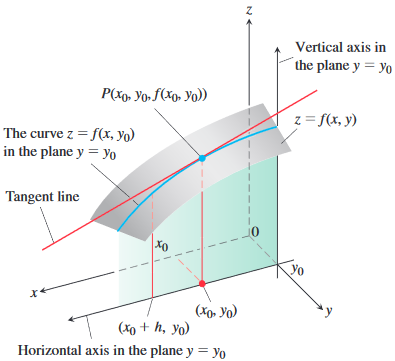
\includegraphics[scale = 0.55]{deriv-parcial-interpretacion-geometrica.png}
\caption{Hass, et al (2019). \textit{Thomas Calculus. Early Transcendentals in SI Units}. Pp. 789.}
\end{figure}

\subsection{Derivada parcial expresada como una función.}

Probablemente ya notamos las similitudes de la derivada parcial con respecto a su par ordinaria. Otra semejanza de ellas es que pueden ser expresadas como funciones. Generalicemos este hecho en su definición del límite.

Las derivadas parciales de $f(x, \ y)$ con respecto a $x$ e $y$ son definidas por las funciones:
\begin{align*}
(1) \ \derivpar{x} f(x, \ y) = \lim_{h \to 0} \frac{f(x + h, \ y) - f(x, \ y)}{h} \\ \\
(2) \ \derivpar{y} f(x, \ y) = \lim_{h \to 0} \frac{f(x, \ y + h) - f(x, \ y)}{h}
\end{align*}
siempre que los límites en (1) y (2) existan.

En (1) se asume que $y$ es constante mientras que $x$ varía en $f(x, \ y)$. Esto conlleva al mismo hecho visto en la sección 2:\footnote{Que también se aplica en (2).}
\[
  \derivpar{x} f(x, \ y) = \deriv{x} f(x, \ y), \ (y = \text{constante})
\]
Por lo tanto, es posible usar las \textbf{reglas de las derivadas ordinarias} (como las del producto, de la cadena, etc) para conocer las derivadas parciales de $f(x, \ y)$ expresadas como función, lo que ayuda a hacer más expedito este proceso que al utilizar la definición del límite.

Si queremos, por ejemplo, calcular el valor de $f_{y}(x_{0}, \ y_{0})$ de una función $f(x, \ y)$ usando las reglas de las derivadas ordinarias, se deben seguir los siguientes pasos:

\begin{enumerate}
\item Obtener la expresión algebraica de $f_{y}(x, \ y)$.
\item Calcular el valor de salida de $f_{y}(x, \ y)$ en $(x_{0}, \ y_{0})$.
\end{enumerate}

\ejemplo Calcule las derivadas parciales de $f(x, \ y) = x \exp(x^{2}y)$ en el punto $(1, \ \ln(2))$.

\solucion Comencemos con la derivada con respecto a $x$ de $f(x, \ y)$, lo que significa que asumimos que $y$ es una constante.
\[
  \derivpar{x} (x \exp(x^{2}y))
\]
Tanto $x$ como $\exp(x^{2}y)$ están variando con respecto a $x$, por lo tanto usemos la regla del producto para calcular esta derivada.
\begin{align*}
  \derivpar{x} (x \exp(x^{2}y)) &= \derivpar{x} x \cdot \exp(x^{2}y) + x \cdot \derivpar{x} \exp(x^{2}y) \\
                                &= \exp(x^{2}y) + x \cdot \left(\derivpar{(x^{2}y)} \exp(x^{2}y) \cdot \derivpar{x} (x^{2}y)\right) \\
                                &= \exp(x^{2}y) + x \cdot \exp(x^{2}y) \cdot 2xy \\
                                &= \exp(x^{2}y) (1 + 2x^{2}y)
\end{align*}
Luego, evaluamos a $f_{x}(x, \ y)$ en $(1, \ \ln(2))$.
\[
  \pderivpar{x}{(x \exp(x^{2}y))}{(1, \ \ln(2))} = \exp((1^{2}) \ln(2)) \cdot (1 + 2(1^{2})(\ln(2)))
                                                 = 2 + 4 \ln(2)
\]
Ahora calculemos $f_{y}(x, \ y)$, la que también puede ser resuelta usando la regla del producto.
\begin{align*}
  \derivpar{y} (x \exp(x^{2}y)) &= \derivpar{y} x \cdot \exp(x^{2}y) + x \cdot \derivpar{y} \exp(x^{2}y) \\
                                &= 0 \cdot \exp(x^{2}y) + x \cdot \left(\derivpar{(x^{2}y)} \exp(x^{2}y) \cdot \derivpar{y} x^{2}y\right) \\
                                &= x \cdot \exp(x^{2}y) \cdot x^{2} \\
                                &= x^{3} \cdot \exp(x^{2}y)
\end{align*}
Finalmente, veamos cuál es el valor de salida de $f_{y}(x, \ y)$ en $(1, \ \ln(2))$.
\[
  \pderivpar{y}{(x \exp(x^{2}y))}{(1, \ \ln(2))} = (1^{3}) \exp(1^{2} \ln(2)) = \exp(\ln(2)) = 2
\]

\ejemplo Calcule las derivadas de
\[
  f(x, \ y) = \frac{2y}{y + \cos(x)}
\]
\solucion Partamos con $f_{x}(x, \ y)$. Al aplicar la regla del cociente, se obtiene que:
\begin{align*}
  \derivpar{x}\left(\frac{2y}{y + \cos(x)}\right) &= \frac{(y + \cos(x)) \cdot f_{x}(2y) - 2y \cdot f_{x}(y + \cos(x))}{(y + \cos(x))^{2}} \\
                                                  &= \frac{-(2y)(-\sin(x))}{(y + \cos(x))^{2}} \\
                                                  &= \frac{2y \sin(x)}{(y + \cos(x))^{2}}
\end{align*}
La derivada de $f(x, \ y)$ con respecto a $y$ también se puede resolver con la regla del cociente.
\begin{align*}
\derivpar{y}\left(\frac{2y}{y + \cos(x)}\right) &= \frac{(y + \cos(x)) \cdot f_{y}(2y) - 2y \cdot f_{y}(y + \cos(x))}{(y + \cos(x))^{2}} \\
                                                &= \frac{2y + 2\cos(x) - 2y}{(y + \cos(x))^{2}} \\
                                                &= \frac{2\cos(x)}{(y + \cos(x))^{2}}
\end{align*}

\ejemplo Considere la ecuación
\[
  yz - \ln(z) = x + y
\]
Asuma que $z$ depende de $x$ e $y$. Calcule su derivada con respecto a $x$ bajo el supuesto de que esta existe.

\solucion La variable $z$ es, \textbf{implícitamente}, una función de $x$ e $y$. Por lo tanto, para obtener su derivada podemos aplicar esta operación en ambos lados de la igualdad\footnote{Técnica conocida también como \textbf{diferenciación implícita}.}.
\begin{align*}
                                                         \derivpar{x}(yz - \ln(z)) &= \derivpar{x}(x + y) \\
\left(y \cdot \derivpar{x}z\right) - \left(\frac{1}{z} \cdot \derivpar{x} z\right) &= 1 \\
                                  \derivpar{x}z \cdot \left(y - \frac{1}{z}\right) &= 1 \\
                                                                     \derivpar{x}z &= \frac{z}{yz - 1}
\end{align*}

\subsection{Derivadas parciales de orden superior y el teorema de Clairaut.}

Así como ocurre con las funciones de una variable, también es posible calcular la derivada de una función multivariada en más de una ocasión. Al conjunto de éstas se conocen como derivadas parciales de orden superior.

La derivada parcial de orden superior se puede calcular con respecto a la variable de la que se obtuvo anteriormente o en relación a otra de las que depende la función original. Todo ese proceso siempre debe ser registrado en su notación.

Por ejemplo, a continuación se expresan todas las \textbf{segundas derivadas parciales} de una función $f(x, \ y)$ (asumiendo que existen). Como se observa en sus lados derechos, la primera que se calcula (es decir, la de primer orden) es la que está adentro del paréntesis.
\begin{align*}
\nderivpar{2}{x} f(x, \ y) &= \derivpar{x} \left(\derivpar{x} f(x, \ y)\right) &
  \nderivpar{2}{y} f(x, \ y) &= \derivpar{y} \left(\derivpar{y} f(x, \ y)\right) \\
\nbiderivpar{2}{x}{y} f(x, \ y) &= \derivpar{y} \left(\derivpar{x} f(x, \ y)\right) &
  \nbiderivpar{2}{y}{x} f(x, \ y) &= \derivpar{x} \left(\derivpar{y} f(x, \ y)\right)
\end{align*}
Las derivadas $\nbiderivpar{2}{x}{y} f(x, \ y)$ y $\nbiderivpar{2}{y}{x} f(x, \ y)$ se conocen como \textbf{derivadas parciales mixtas} de $f(x, \ y)$ y también pueden expresarse como:
\begin{align*}
  f_{xy}(x, \ y) &= (f_{x}(x, \ y))_{y} = f_{xy} = (f_{x})_{y} \\
  f_{yx}(x, \ y) &= (f_{y}(x, \ y))_{x} = f_{yx} = (f_{y})_{x}
\end{align*}
En el caso de las derivadas parciales mixtas de una función en un punto, es posible encontrar una útil igualdad llamada \textbf{teorema de Clairaut} que fue planteada por el matemático francés Alexis Clairaut en el siglo XVIII. Esta señala que si una función real $f(x, \ y)$ y sus derivadas parciales $f_{x}$, $f_{y}$, $f_{xy}$ y $f_{yx}$:

\begin{enumerate}
\item Están definidas en una región abierta $D \subseteq \R^{2}$ en la que un punto $(x_{0}, \ y_{0}) \in D$.
\item Son \textbf{continuas} en $(x_{0}, \ y_{0})$.
\end{enumerate}

entonces:
\[
  f_{xy}(x_{0}, \ y_{0}) = f_{yx}(x_{0}, \ y_{0})
\]
El teorema de Clairaut también se aplica a las derivadas parciales mixtas de funciones de $n$ variables ($n > 2$), así como en aquellas que son continuas en todo su dominio.

\ejemplo La siguiente ecuación diferencial parcial se conoce como la ``ecuación de onda'' (\textit{wave equation}).
\[
  \nderivpar[u]{2}{t} = a^{2} \left(\nderivpar[u]{2}{x}\right) \qquad (a \in \R_{0}^{+})
\]
Verifique que la función $u(x, \ t) = \sin(x - at)$ es una solución de la ecuación de onda.

\solucion Comencemos calculando la segunda derivada parcial de $u(x, \ t)$ con respecto a $x$.
\begin{align*}
      \derivpar[u]{x} &= \derivpar{x}(\sin(x - at)) = \cos(x - at) \cdot 1 = \cos(x - at) \\
  \nderivpar[u]{2}{x} &= \derivpar{x} \cos(x - at) = - \sin(x - at) \cdot 1 = -\sin(x - at)
\end{align*}
Ahora resolvamos $u_{tt}(x, \ t)$.
\begin{align*}
      \derivpar[u]{t} &= \derivpar{t}(\sin(x - at)) = \cos(x - at) \cdot (-a) = -a \cdot \cos(x - at) \\
  \nderivpar[u]{2}{t} &= \derivpar{t}(-a \cdot \cos(x - at)) = (-a) \cdot (-\sin(x - at)) \cdot (-a) = a^{2} \cdot (-\sin(x - at))
\end{align*}

Puesto que $\nderivpar[u]{2}{x} = -\sin(x - at)$, se puede concluir y verificar que:
\[
  \nderivpar[u]{2}{t} = a^{2} \left(\nderivpar[u]{2}{x}\right)
\]

\ejemplo Demuestre que la función $u(x, \ y) = \exp(x) \cdot \sin(y)$ es una solución de la ecuación de Laplace.
\[
  \nderivpar[u]{2}{x} + \nderivpar[u]{2}{y} = 0
\]
\solucion Partamos con las primeras derivadas de $u(x, \ y)$ con respecto a $x$ e $y$.
\begin{align*}
  \derivpar[u]{x} &= \derivpar{x} (\exp(x) \cdot \sin(y)) & \derivpar[u]{y} &= \derivpar{y}(\exp(x) \cdot \sin(y)) \\
                  &= \exp(x) \cdot \sin(y)                &                 &= \exp(x) \cdot \cos(y)
\end{align*}
Luego, calculemos a $u_{xx}$ y $u_{yy}$.
\begin{align*}
  \nderivpar[u]{2}{x} &= \derivpar{x} (\exp(x) \cdot \sin(y)) & \nderivpar[u]{2}{y} &= \derivpar{y} (\exp(x) \cdot \cos(y)) \\
                      &= \exp(x) \cdot \sin(y)                &                     &= - \exp(x) \cdot \sin(y)
\end{align*}
Finalmente, sumemos las dos segundas derivadas parciales de $u(x, \ y)$.
\[
  \nderivpar[u]{2}{x} + \nderivpar[u]{2}{y} = \exp(x) \cdot \sin(y) + (-\exp(x) \cdot \sin(y)) = 0
\]
Por lo tanto, se confirma que $u(x, \ y) = \exp(x) \cdot \sin(y)$ satisface a la ecuación de Laplace\footnote{En particular, las soluciones de esta ecuación diferencial parcial se llaman \textbf{funciones harmónicas}.}.

\end{document}